\Transcb{yellow}{blue}{Transient cosmic sources}
\twocolumn
\begin{center}
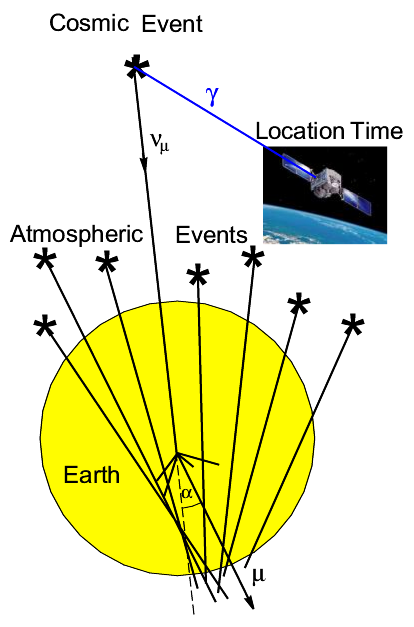
\includegraphics[keepaspectratio,height=15cm]{atm-bkg}
\end{center}

\newpage

\begin{itemize}
\item No signal $\rightarrow$ Give flux upper limit
\item Link observations and flux via Effective area
\item[] $ A_{eff} \equiv$ obs. event rate~/~incoming flux
\item[] $\rightarrow$ Flux limit = max. event rate~/~$A_{eff}$
\end{itemize}
%
\begin{center}
{\blue $\nu_{\mu}+\bar{\nu}_{\mu}$ Effective area (solid angle averaged)}\\
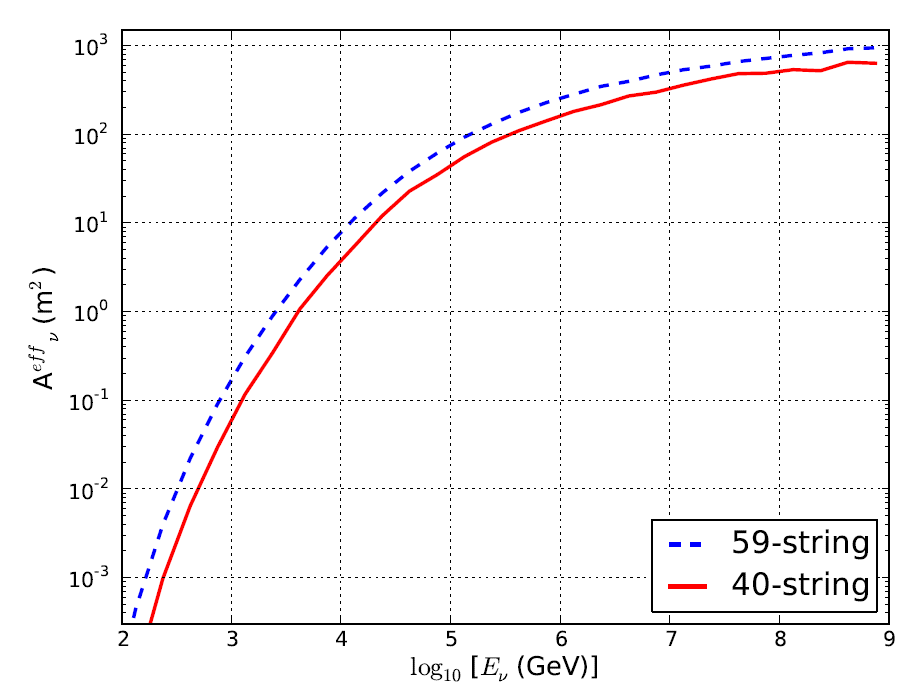
\includegraphics[keepaspectratio,height=9.5cm]{ic59+40-eff-area}
\end{center}

\Tr
\twocolumn
\begin{center}
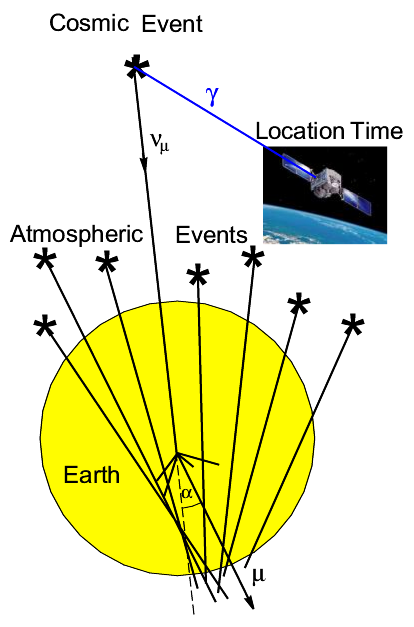
\includegraphics[keepaspectratio,height=15cm]{atm-bkg}
\end{center}

\newpage

\begin{center}
{\red IceCube GRB prompt $\nu$ flux limit}\\
{\large [ApJ Let. 805 (2015) L5]}\\
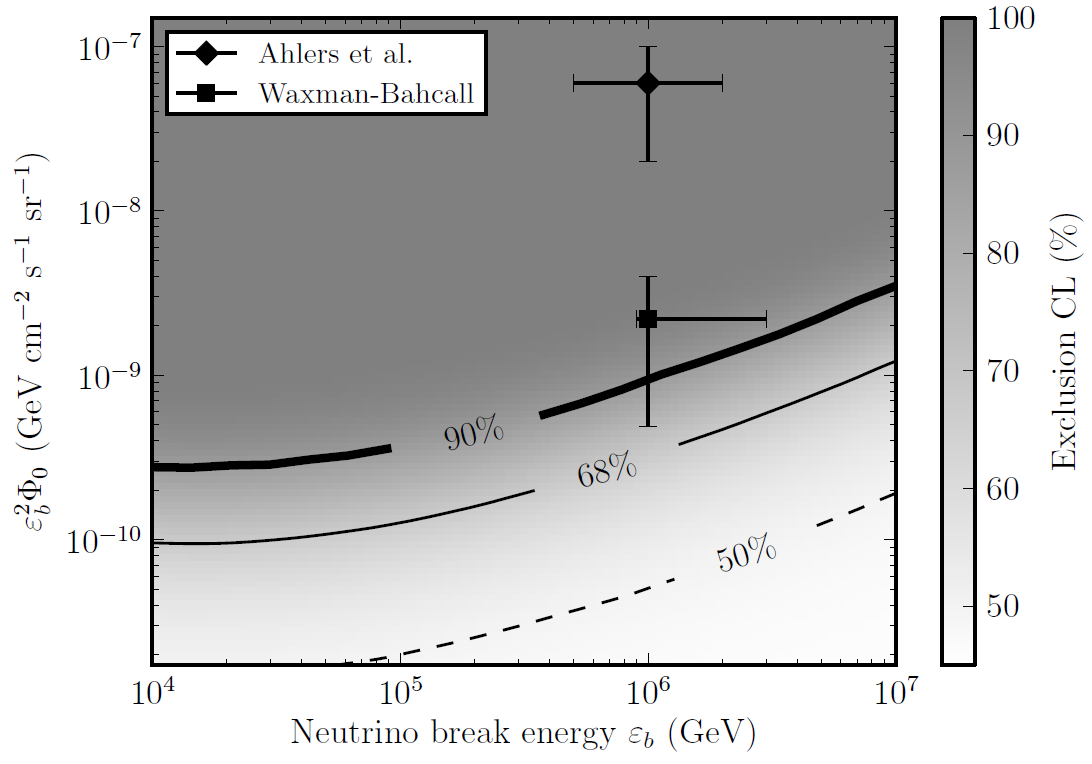
\includegraphics[keepaspectratio,width=13cm]{ic-grb-limit-prompt}
\end{center}
\begin{itemize}
\item[] GRBs not the (only) UHECR sources
\item[] {\blue Or :} $\nu$ prod. lower than expected
\item[] {\blue Or :} $\nu$ prod. outside prompt phase
\end{itemize}
